\documentclass{article}
\usepackage{graphicx}
\usepackage{amsmath}

\begin{document}

\title{Problem 17 - Arctangent function by numerical root finding}
\author{Jens S. K. Jensen}
\date{\today}
\maketitle

\section{Introduction}
This report covers a numerical implementation of the arctangent function
\begin{equation}
	a = arctan(x),
	\label{eq:atan1}
\end{equation}
by finding roots of the equation
\begin{equation}
	tan(a) - x = 0.
	\label{eq:tan}
\end{equation}
That is, given $x$ find $a$ via eq. (\ref{eq:tan}).

\section{Implementation}
The numerical solution is implemented via a root-finding algorithm in GSL, in this case the \textit{gsl\_multiroot\_fsolver\_hybrids} solver was used, which relies on finite differences for derivatives. However, the better option would be to employ an algorithm using analytical derivatives, since the derivative of $tan(a)$ is known as $1+tan(a)^2$. For this small problem though, the derivative-free solver was judged adequate.

The solver relies on a starting point (henceforth called $a_0$), which if not chosen carefully can lead to undesirable results. All root-finding algorithms in the GSL library uses some variant of the newton iteration
\begin{equation}
	x_1 = x_0 - J(x_0)^{-1}f(x_0),
\end{equation}
with $x_0$ and $f(x_0)$ being vector quantities and $J(x_0)$ being the Jacobian matrix of the system. Looking at figure ?? we see why we must choose $a_0$ with care. For instance, setting $a_0 = 0$ is fine for small values of $x$, but will result in a large error for the final value of $a$ as $x$ exceeds $\pm \pi$ (for $a_0=0$), since the $arctan$ function only is defined for the initial repetition of the tangent function
\begin{equation}
	x = tan(a) \quad -\frac{\pi}{2}<a<\frac{\pi}{2}.
\end{equation}



\section{Plot visualization}


\begin{figure}
	\centering
	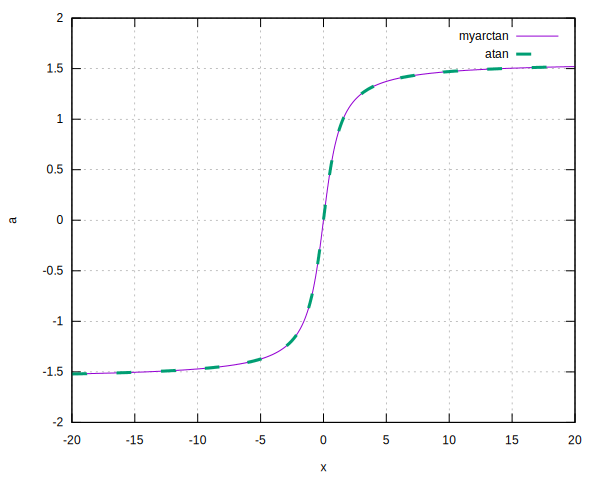
\includegraphics{plot.pdf}
	\caption{Visualization of the arctan function, showing both own numerical (myarctan) and the atan definition from math.h}
	\label{fig:plot}
\end{figure}

\end{document}
